\documentclass[letterpaper,12pt]{extarticle}
\PassOptionsToPackage{hidelinks}{hyperref}
\usepackage{astro-mini}
\usepackage{booktabs}

\usepackage{array}
\newcolumntype{L}{>{$}l<{$}}
\newcolumntype{C}{>{$}c<{$}}
\newcolumntype{R}{>{$}r<{$}}

% Busca imágenes tanto en el directorio raíz del proyecto como en img/
\graphicspath{{../}{img/}}

\begin{document}

% ============================================================
%  PORTADA
% ============================================================
\begin{center}
    \Large \textbf{Clasificación Supervisada de Estrellas Variables\\
    con Bosques Aleatorios}

    \vspace{4mm}
    \large Juan David Aparicio Gutiérrez

    \vspace{2mm}
    \normalsize Universidad de los Andes --- Astrofísica Observacional con Machine Learning
\end{center}

\vspace{2mm}

% ============================================================
%  RESUMEN
% ============================================================
\begin{abstract}
Se presenta la clasificación supervisada de 6\,366 estrellas variables del
relevamiento OGLE-IV en cuatro categorías: binarias, variables de período largo
(LPV), pulsantes y otras. Partiendo únicamente de series de tiempo fotométricas
en las bandas $I$ y $V$, se construyeron y evaluaron nueve features estadísticos
mediante histogramas por clase. Tras la exploración se retuvieron cuatro: el
color calculado con el estimador de biweight location $(V-I)_{BW}$, el
logaritmo del período obtenido con Lomb-Scargle a partir de la curva de luz en
banda $I$, la asimetría y la amplitud fotométrica. Un clasificador de bosque
aleatorio con estos cuatro features alcanzó una exactitud global del 91.2\%, con
el mejor desempeño para las LPV (F1\,=\,0.962).
\end{abstract}

% ============================================================
%  1. INTRODUCCIÓN / MARCO TEÓRICO
% ============================================================
\section{Introducción}

El estudio de estrellas variables ocupa un lugar central en la astrofísica
moderna: su variabilidad fotométrica revela propiedades físicas como radio,
temperatura efectiva, período de pulsación y geometría orbital. Con el advenimiento
de grandes relevamientos fotométricos, la cantidad de curvas de luz disponibles
crece más rápido que la capacidad de clasificarlas manualmente, lo que motiva el
uso de técnicas de aprendizaje automático supervisado.

En este trabajo se aplica un clasificador de bosque aleatorio para distinguir
cuatro tipos de estrellas variables a partir de features estadísticos derivados
\textit{exclusivamente} de las curvas de luz en las bandas $I$ y $V$, sin
utilizar ningún parámetro previo del catálogo como feature.

% -----------------------------------------------------------
\subsection{Los datos}
% -----------------------------------------------------------

Los datos provienen del Experimento de Lente Gravitacional Óptica en su cuarta
fase (OGLE-IV; \citealt{udalski2015}), uno de los relevamientos fotométricos de
largo plazo más exhaustivos del hemisferio sur. OGLE-IV opera con el telescopio
de 1.3\,m de Varsovia en el Observatorio de Las Campanas (Chile) y ha monitoreado
millones de estrellas durante más de una década con cadencias de muestreo que van
de días a semanas.

Para este trabajo se utilizaron curvas de luz de los campos LMC562 y LMC563,
correspondientes a regiones de la Nube Mayor de Magallanes (LMC) observadas en
las bandas fotométricas $I$ (infrarrojo cercano, $\lambda_\text{ef}\approx
806$\,nm) y $V$ (visual, $\lambda_\text{ef}\approx 551$\,nm). Cada estrella
cuenta con una serie de tiempo de magnitud aparente en función del tiempo
heliocéntrico juliano (HJD), con su incertidumbre fotométrica asociada.

Todos los features del modelo se extraen directamente de las curvas de luz; el
catálogo se utiliza únicamente para las etiquetas de clase. El único criterio de
exclusión es la no disponibilidad simultánea de curva de luz en ambas bandas, más
tres clases de muy escasa representación estadística (T2CEP, ACER y ACEP). La
\textbf{muestra de trabajo} queda compuesta por \textbf{6\,366 estrellas}.

% -----------------------------------------------------------
\subsection{Tipos de estrellas variables}
% -----------------------------------------------------------

Las estrellas variables se clasifican de acuerdo con el mecanismo físico que
origina su variabilidad \citep{samus2017, Karttunen2016}. En este trabajo se
trabaja con cuatro categorías:

\textbf{Binarias (BINARY).} Un sistema binario está formado por dos estrellas que
orbitan en torno a su centro de masa común \citep{Karttunen2016}. La variabilidad
fotométrica puede producirse por dos mecanismos: en las \textit{binarias en eclipse}
(ECL), uno de los componentes pasa periódicamente frente al otro bloqueando
parcialmente su luz; en las \textit{elipsoidales} (ELL), la deformación de marea
genera variaciones de flujo sin eclipse \citep{pawlak2016, Soszynski2016}. Sus
períodos van desde pocas horas hasta decenas de días. La muestra incluye
1\,434 binarias.

\textbf{Variables de período largo (LPV).} Son gigantes rojas en estados avanzados
de evolución estelar cuya variabilidad se origina en pulsaciones radiales de gran
amplitud. Incluyen las estrellas tipo Mira, semirregulares y otras variables lentas
\citep{mattei1997, soszynski2009lpv}. Sus períodos típicamente superan los 100 días
y sus amplitudes son de las mayores observadas. Es la clase más numerosa de la
muestra: 2\,607 estrellas.

\textbf{Pulsantes (PULSATING).} Agrupa tres subtipos bien estudiados: las
\textit{RR Lyrae} (RRLYR), con períodos entre 0.2 y 1 día \citep{Soszynski2009};
las \textit{cefeidas clásicas} (DCEP), con períodos de 1 a 100 días y la famosa
relación período-luminosidad de Leavitt \citep{Soszynski2008}; y las \textit{Delta
Scuti} (DSCT), variables pulsantes de baja amplitud y rápida variación
\citep{Pietrukowicz2013}. En los tres casos el mecanismo de ionización del helio
sostiene la pulsación. La muestra incluye 913 pulsantes.

\textbf{Otras (OTHER).} Categoría heterogénea que agrupa objetos cuya variabilidad
no corresponde a ninguna de las clases anteriores (p.~ej., Be, T Tauri u otras
variables de naturaleza incierta). Son 1\,412 estrellas.

% -----------------------------------------------------------
\subsection{Bosques aleatorios}
% -----------------------------------------------------------

Un bosque aleatorio (\textit{Random Forest}) es un clasificador de ensamble
propuesto por \citet{breiman2001} que combina múltiples árboles de decisión
entrenados de forma independiente. Cada árbol se construye sobre una muestra con
reemplazo (\textit{bootstrap}) del conjunto de entrenamiento, introduciendo
variabilidad entre árboles. En cada nodo de división solo se considera un
subconjunto aleatorio de $\lfloor\sqrt{p}\rfloor$ features candidatos (donde $p$
es el total), descorrelacionando los árboles. La predicción final se obtiene por
votación mayoritaria.

La combinación de \textit{bagging} y selección aleatoria de features reduce la
varianza sin aumentar el sesgo, haciéndolo robusto frente al sobreajuste.

Una propiedad adicional valiosa es la \textbf{importancia de Gini} (también
denominada \textit{Mean Decrease in Impurity}, MDI). Para definirla, se parte
de la impureza de Gini \citep{breiman1984} de un nodo $t$ con $n_t$ muestras
distribuidas entre $K$ clases:
\begin{equation}\label{eq:gini}
    G(t) = 1 - \sum_{k=1}^{K} \hat{p}_{tk}^{\,2},
\end{equation}
donde $\hat{p}_{tk}$ es la fracción de muestras de clase $k$ en el nodo.
Un nodo perfectamente puro tiene $G=0$; un nodo con mezcla uniforme alcanza
el máximo $G = 1 - 1/K$. Cuando se divide el nodo $t$ en dos hijos $t_L$
y $t_R$, la reducción de impureza asociada a esa división es
\begin{equation}\label{eq:delta_gini}
    \Delta G(t) = G(t)
                 - \frac{n_{t_L}}{n_t}\,G(t_L)
                 - \frac{n_{t_R}}{n_t}\,G(t_R).
\end{equation}
La importancia del feature $j$ se obtiene acumulando estas reducciones,
ponderadas por la proporción de muestras que pasan por cada nodo, a lo largo
de todos los árboles del bosque \citep{breiman2001}:
\begin{equation}\label{eq:mdi}
    \mathrm{MDI}(j) =
        \frac{1}{|\mathcal{T}|}
        \sum_{T\,\in\,\mathcal{T}}\;
        \sum_{\substack{t\,\in\,T \\ v(t)=j}}
        \frac{n_t}{n}\,\Delta G(t),
\end{equation}
donde $\mathcal{T}$ es el conjunto de árboles, $v(t)$ es el feature empleado
en la división del nodo $t$ y $n$ es el tamaño del conjunto de entrenamiento.
Las puntuaciones resultantes se normalizan para que sumen la unidad. Un feature
que separa consistentemente las clases en muchos nodos acumula una puntuación
alta independientemente de la profundidad en que ocurra la división.

Se utilizó la implementación de \texttt{scikit-learn} \citep{sklearn2011} con
500 árboles y semilla aleatoria fija para reproducibilidad.\footnote{El código
completo de este trabajo está disponible en
\href{https://github.com/juand4g/AstroML_202610/tree/main/Trabajo\%20final}%
{\texttt{github.com/juand4g/AstroML\_202610}}.}

% ============================================================
%  2. OBJETIVOS
% ============================================================
\section{Objetivos}

\begin{enumerate}
    \item Construir un conjunto de features estadísticos derivados exclusivamente
    de series de tiempo fotométricas en las bandas $I$ y $V$ para la
    caracterización de curvas de luz de estrellas variables.

    \item Evaluar el poder discriminante de cada feature mediante histogramas
    superpuestos por clase y seleccionar un subconjunto representativo para la
    clasificación.

    \item Entrenar y evaluar un clasificador de bosque aleatorio para la
    clasificación supervisada de cuatro tipos de estrellas variables a partir de
    los features seleccionados.

    \item Analizar la importancia relativa de los features seleccionados e
    identificar los más informativos para la tarea de clasificación.
\end{enumerate}

% ============================================================
%  3. METODOLOGÍA
% ============================================================
\section{Metodología}

\subsection{Exploración y definición de features}

Se evaluó un conjunto de nueve features candidatos. Para cada uno se generó un
histograma superpuesto por clase, comparando visualmente las distribuciones de
las cuatro categorías (Fig.~\ref{fig:histogramas}). A continuación se define cada
feature explorado.

\begin{figure}[H]
    \centering
    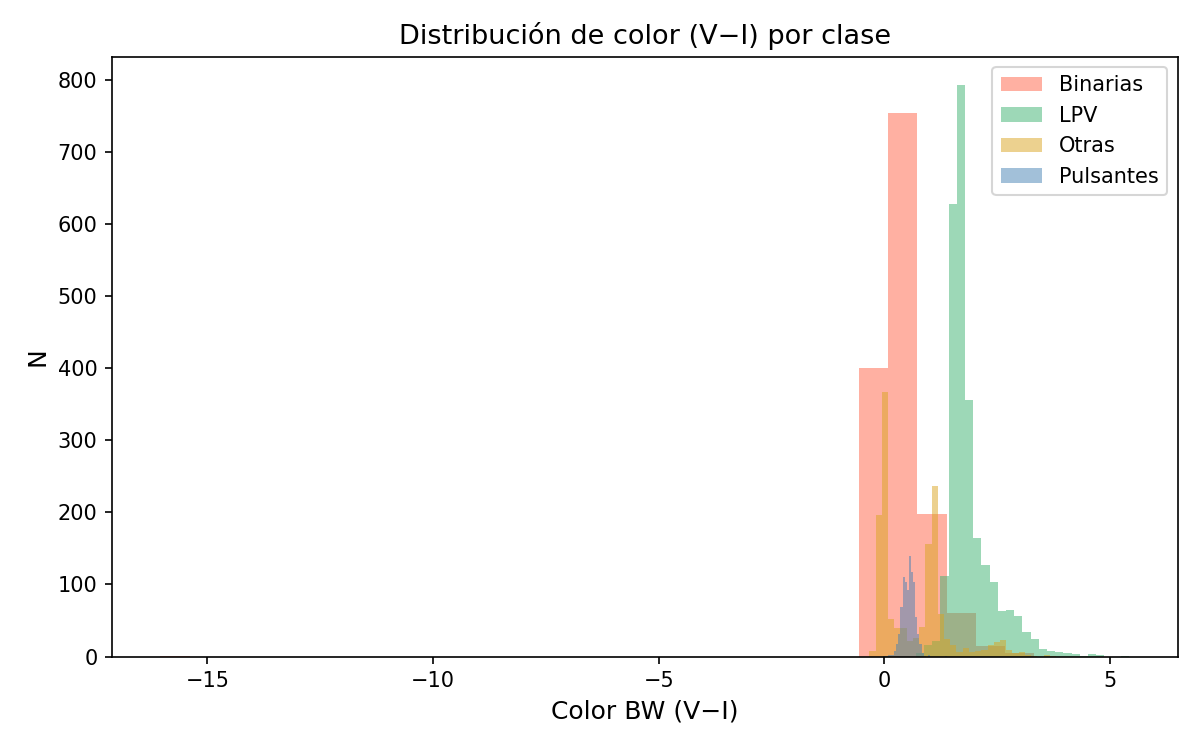
\includegraphics[width=0.48\textwidth]{histogram_colour_bw_by_class.png}
    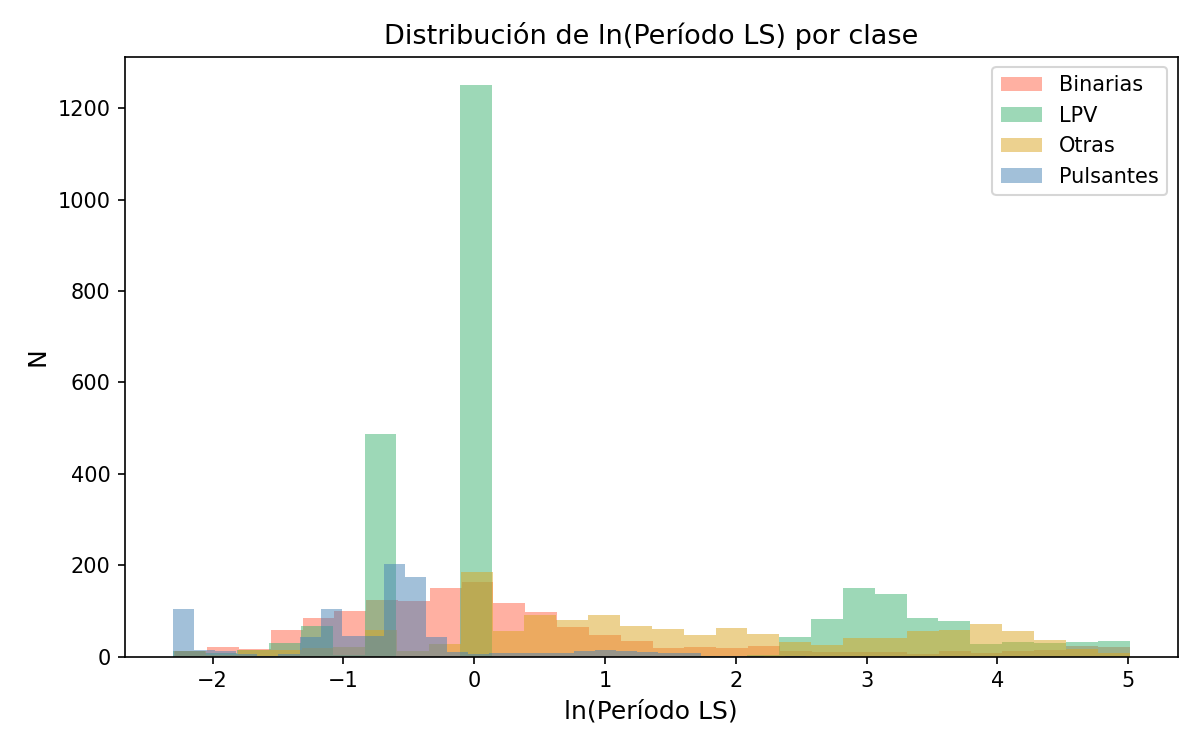
\includegraphics[width=0.48\textwidth]{histogram_lnP_ls_by_class.png}\\[4pt]
    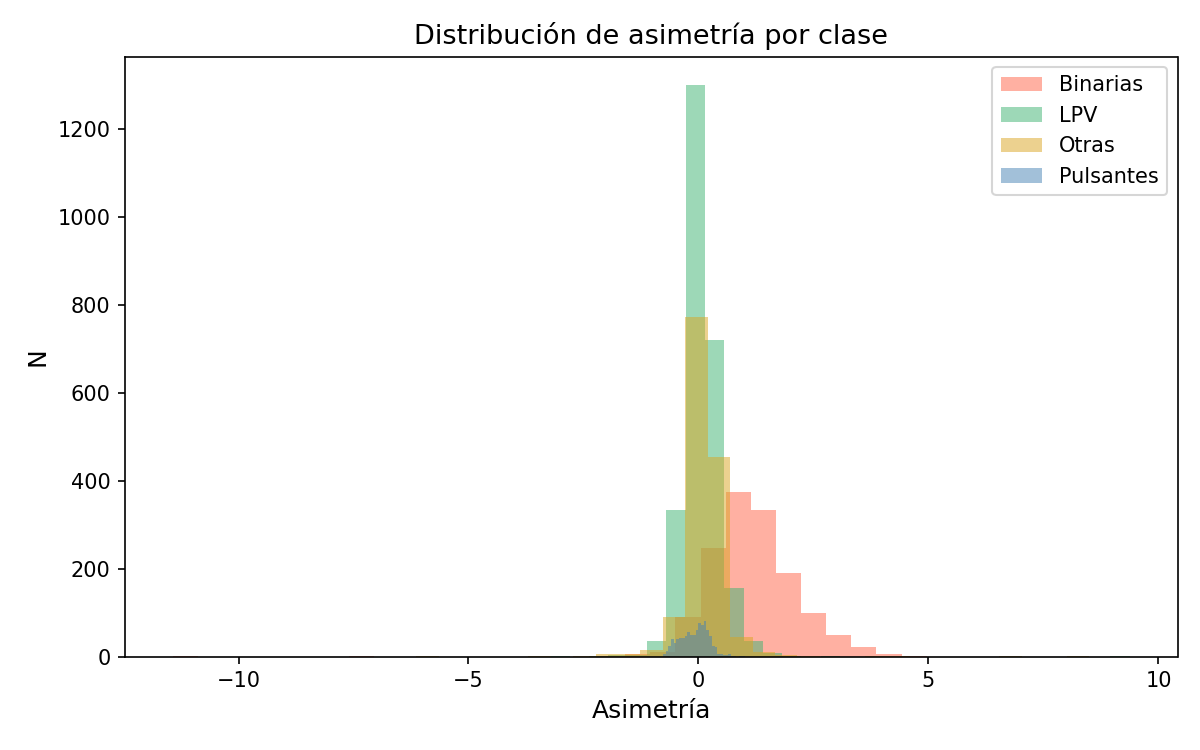
\includegraphics[width=0.48\textwidth]{histogram_skew_lc_by_class.png}
    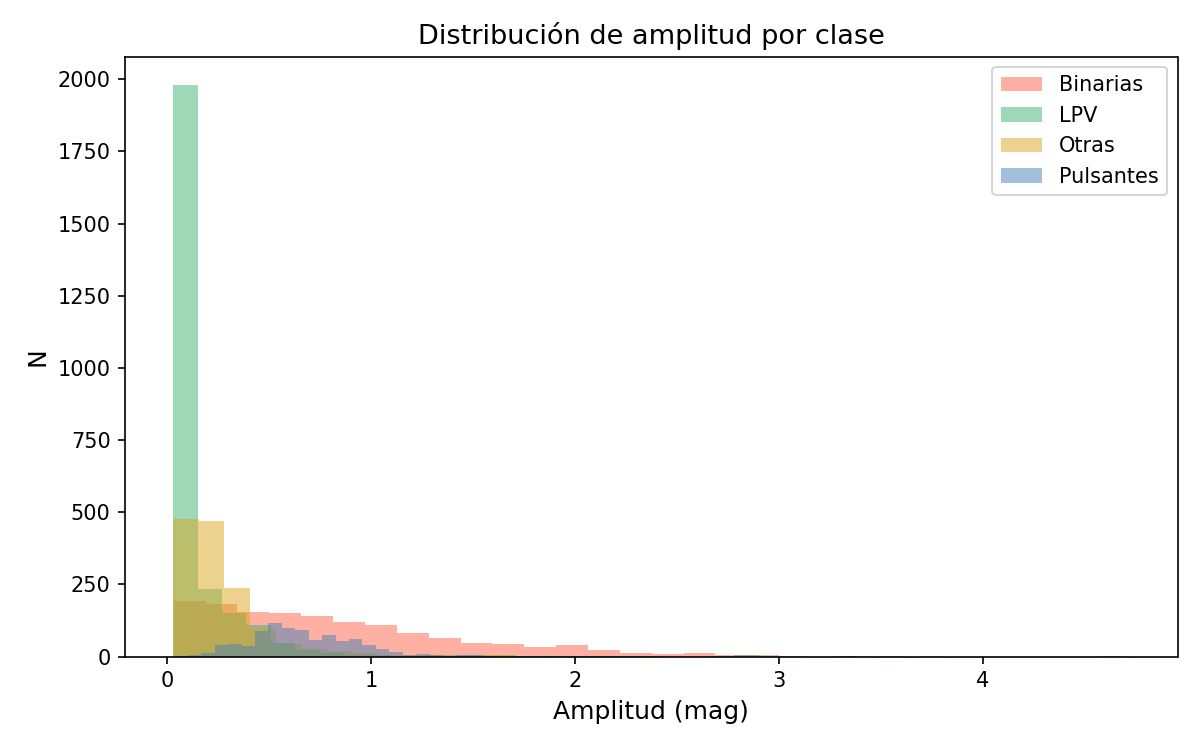
\includegraphics[width=0.48\textwidth]{histogram_amp_lc_by_class.png}
    \caption{Distribución de los cuatro features retenidos para cada clase.
    \textit{Arriba izq.:} color biweight $(V-I)_{BW}$.
    \textit{Arriba der.:} logaritmo del período calculado con Lomb-Scargle.
    \textit{Abajo izq.:} asimetría de la curva de luz en banda $I$.
    \textit{Abajo der.:} amplitud fotométrica en banda $I$.
    Las LPV se distinguen por su color más rojo y sus amplitudes y períodos mayores.}
    \label{fig:histogramas}
\end{figure}

\textbf{Amplitud ($A$).} Diferencia entre la magnitud más tenue y la más brillante
en la curva de luz en banda $I$:
\begin{equation}
    A = m_{\max} - m_{\min}.
\end{equation}
Cuantifica el rango de variación fotométrica. Las LPV muestran amplitudes
típicamente superiores a 0.5\,mag.

\textbf{Asimetría (\textit{skewness}, $\gamma_1$).} Tercer momento estadístico
estandarizado de la distribución de magnitudes:
\begin{equation}
    \gamma_1 = \frac{E\!\left[(m - \bar{m})^3\right]}{\sigma^3}.
\end{equation}
Una distribución simétrica tiene $\gamma_1 = 0$. Las pulsantes y binarias muestran
asimetrías características relacionadas con la forma de sus curvas de luz.

\textbf{Curtosis ($\gamma_2$).} Cuarto momento estandarizado (exceso):
\begin{equation}
    \gamma_2 = \frac{E\!\left[(m - \bar{m})^4\right]}{\sigma^4} - 3.
\end{equation}
Aunque explorado, no fue incluido en el modelo final por su aportación marginal y su relación tan estrecha con la asimetría.

\textbf{Magnitud media.} Promedio de la magnitud en banda $I$. Descartada como
feature; véase la Sección~\ref{sec:problemas}.

\textbf{Estadístico KPSS.} Estadístico de la prueba de estacionariedad de
Kwiatkowski-Phillips-Schmidt-Shin \citep{kwiatkowski1992} sobre la serie temporal
de magnitudes. Los histogramas no mostraron separación apreciable entre clases y
fue descartado.

\textbf{Tasa de extremos locales.} Proporción de puntos de la curva de luz que son
extremos locales, estimada como el número de cambios de signo en la diferencia
discreta $\Delta m_i = m_{i+1}-m_i$ dividido por la longitud de la serie. La
distribución resultó similar para todas las clases y fue descartada.

\textbf{Color biweight $(V-I)_{BW}$.} Diferencia entre el estimador de biweight
location de las magnitudes en banda $V$ y en banda $I$:
\begin{equation}
    (V-I)_{BW} = T_{BW}(V) - T_{BW}(I).
\end{equation}
El biweight location \citep{beers1990} es un estimador robusto de tendencia central.
Dado un conjunto de magnitudes $\{m_i\}$ con mediana $M$ y desviación absoluta de
la mediana $S$, se definen pesos normalizados $u_i = (m_i-M)/(c\,S)$. El estimador
resulta:
\begin{equation}\label{eq:bw}
    T_{BW} = M + \frac{\displaystyle\sum_{|u_i|<1}(m_i-M)(1-u_i^2)^2}
                      {\displaystyle\sum_{|u_i|<1}(1-u_i^2)^2},
\end{equation}
con constante de ajuste $c=9$. Las mediciones más alejadas que $c\,S$ de la mediana
reciben peso nulo, lo que lo hace resistente a valores atípicos como puntos
contaminados por rayos cósmicos o artefactos de reducción fotométrica. El color
refleja la temperatura efectiva de la estrella y no depende de la distancia.

\textbf{$\ln P_{LS}$.} Logaritmo natural del período dominante calculado de la
curva de luz en banda $I$ mediante el periodograma de Lomb-Scargle
\citep{lomb_1976, scargle_1982}. El periodograma ajusta, para cada frecuencia de
prueba $\nu_k$, una sinusoide a los datos no uniformemente muestreados por mínimos
cuadrados y computa una potencia espectral normalizada; la frecuencia de máxima
potencia define el período adoptado $P_{LS} = 1/\nu_{k^\star}$. Se evaluaron
20\,000 frecuencias en el rango 0.1--150 días.

\subsection{Selección final y entrenamiento}

Tras la exploración visual se conservaron cuatro features: color biweight
$(V-I)_{BW}$, $\ln P_{LS}$, asimetría y amplitud. El conjunto de datos se dividió
en 80\,\% para entrenamiento y 20\,\% para evaluación con estratificación por
clase. Se entrenó un bosque aleatorio con 500 árboles.

% ============================================================
%  4. PROBLEMAS PRESENTADOS Y SOLUCIONES APLICADAS
% ============================================================
\section{Problemas presentados y soluciones aplicadas}
\label{sec:problemas}

\textbf{El desafío del \textit{feature engineering}.}
Uno de los aspectos más críticos del trabajo fue decidir qué información extraer
de las curvas de luz. En una primera exploración, el catálogo OGLE reporta el
período fotométrico para la mayoría de las estrellas, lo que podría simplificar
la tarea si se usara directamente. Sin embargo, en un escenario real donde solo
se dispone de la serie temporal de magnitud versus tiempo, el período debe
calcularse desde cero mediante periodogramas como el de Lomb-Scargle
\citep{lomb_1976, scargle_1982} o el de mínima entropía \citep{cincotta_1995},
cuya fiabilidad depende de la calidad y densidad de muestreo. La elección de qué
estadísticos adicionales extraer para capturar las particularidades de cada tipo
de variabilidad requiere comprensión del dominio y múltiples iteraciones de
exploración y descarte.

La recuperación del período con Lomb-Scargle, evaluada comparando $P_{LS}$ con
el período de catálogo para las estrellas que lo tienen disponible, alcanzó el
63.7\,\% global (con tolerancia $\pm$5\,\%, incluyendo mitad y doble período).
El desglose por clase revela una asimetría marcada: Binarias (92.2\,\%), Pulsantes
(87.2\,\%), Otras (88.8\,\%) y LPV (27.0\,\%). La baja recuperación en las LPV
ocurre porque sus períodos suelen superar los 150 días (el límite superior del
rango de búsqueda), de modo que Lomb-Scargle identifica armónicos u otras señales
espurias. Pese a ello, las LPV son la clase mejor clasificada del modelo (F1\,=\,0.962),
lo que demuestra que el color biweight y la amplitud son suficientemente
discriminantes incluso cuando el período calculado es incorrecto.

\textbf{La magnitud como feature.}
La magnitud media en banda $I$ resulta tentadora porque los diagramas
color-magnitud muestran separación entre clases (las LPV son sistemáticamente
más brillantes en $I$ por ser gigantes rojas de gran luminosidad). No obstante,
la magnitud aparente depende simultáneamente de la luminosidad intrínseca, la
distancia y la extinción interestelar, factores independientes del tipo de
variabilidad. Usar la magnitud como feature introduciría sesgos espurios: dos
estrellas del mismo tipo, situadas a distancias diferentes, se verían
fotométricamente distintas. El color $(V-I)_{BW}$, al ser una diferencia entre
magnitudes en dos bandas, es mayormente un observable intrínseco y no depende de
la distancia, por lo que constituye un sustituto robusto.

% ============================================================
%  5. RESULTADOS
% ============================================================
\section{Resultados}

El modelo de cuatro features alcanzó una \textbf{exactitud global del 91.2\,\%}
sobre el conjunto de evaluación (1\,273 estrellas). La Tabla~\ref{tab:metricas}
resume las métricas por clase; la Figura~\ref{fig:importancias} muestra la
importancia de cada feature según el criterio de Gini, y la
Figura~\ref{fig:confusion} presenta la matriz de confusión.

\begin{table}[H]
    \centering
    \caption{Métricas de clasificación por clase del modelo final con cuatro
    features. El soporte indica el número de estrellas en el conjunto de evaluación.}
    \label{tab:metricas}
    \begin{tabular}{lcccc}
        \toprule
        Clase       & Precisión & Exhaustividad & F1    & Soporte \\
        \midrule
        Binarias    & 0.898     & 0.829         & 0.862 & 287 \\
        LPV         & 0.943     & 0.983         & 0.962 & 521 \\
        Otras       & 0.849     & 0.837         & 0.843 & 282 \\
        Pulsantes   & 0.936     & 0.956         & 0.946 & 183 \\
        \midrule
        Prom. pond. & 0.911     & 0.912         & 0.911 & 1273 \\
        \bottomrule
    \end{tabular}
\end{table}

\begin{figure}[H]
    \centering
    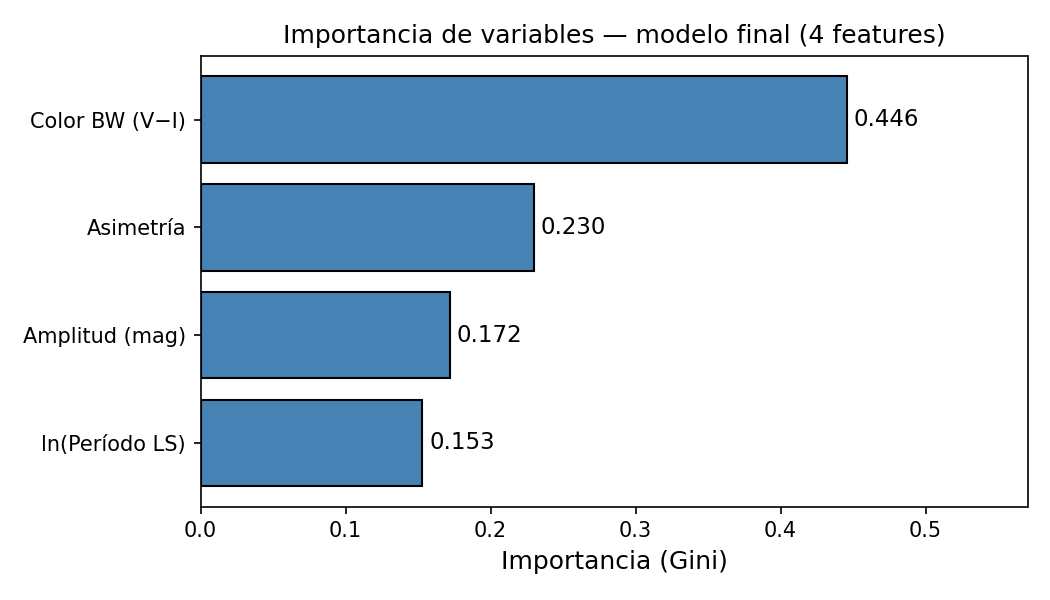
\includegraphics[width=0.72\textwidth]{rf_final4_importances.png}
    \caption{Importancia de cada variable según el criterio de Gini, promediada
    sobre los 500 árboles. El color biweight $(V-I)_{BW}$ es la variable más
    discriminante (Gini\,=\,0.446), seguida de la asimetría (0.230), la amplitud
    (0.172) y el logaritmo del período LS (0.153).}
    \label{fig:importancias}
\end{figure}

\begin{figure}[H]
    \centering
    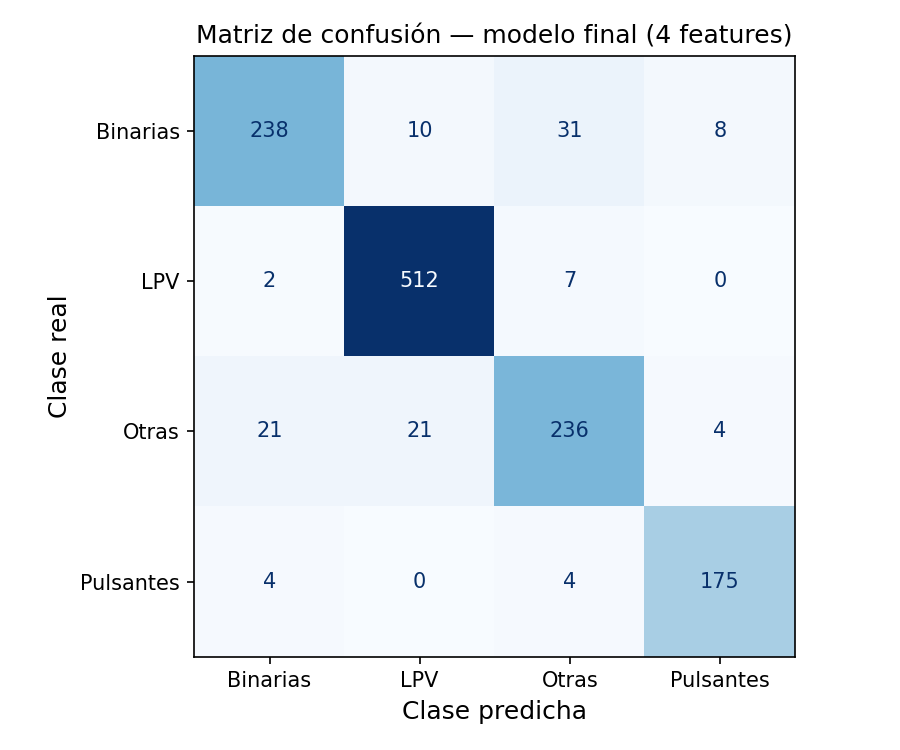
\includegraphics[width=0.56\textwidth]{rf_final4_confusion.png}
    \caption{Matriz de confusión del modelo final sobre el conjunto de evaluación
    (1\,273 estrellas). Cada celda indica el número de estrellas predichas como la
    clase de la columna siendo realmente de la clase de la fila.}
    \label{fig:confusion}
\end{figure}

El color biweight $(V-I)_{BW}$ es el feature más informativo (importancia Gini
= 0.446), seguido de la asimetría (0.230), la amplitud (0.172) y el logaritmo del
período LS (0.153). La mayor importancia del color respecto al período refleja un
resultado notable: incluso cuando el período calculado es impreciso (como ocurre
para las LPV), las propiedades de la distribución de magnitudes bastan para
discriminar las clases.

Las LPV y las Pulsantes obtienen las métricas más altas. Las Binarias y las Otras
muestran el mayor solapamiento mutuo: las binarias elipsoidales pueden presentar
curvas de luz relativamente suaves que se confunden con las de la clase Otras,
mientras que esta última agrupa objetos heterogéneos sin un patrón fotométrico
único.

% ============================================================
%  6. CONCLUSIONES
% ============================================================
\section{Conclusiones}

\begin{enumerate}
    \item Un bosque aleatorio con cuatro features derivados íntegramente de las
    curvas de luz ---color biweight $(V-I)_{BW}$, $\ln P_{LS}$, asimetría y
    amplitud--- clasifica estrellas variables del catálogo OGLE-IV con una
    exactitud global del 91.2\,\%, demostrando que la estructura fotométrica de
    las series de tiempo codifica información suficiente para distinguir los
    principales tipos de variabilidad.

    \item El color biweight $(V-I)_{BW}$ resultó ser el feature más importante
    (Gini = 0.446), indicando que la temperatura efectiva de la estrella es el
    discriminante primario entre clases. Las LPV, como gigantes rojas muy frías,
    presentan colores marcadamente más rojos que el resto.

    \item La selección de features es el paso más crítico del proceso. La
    exploración sistemática permitió descartar la magnitud media (dependiente de
    la distancia), el estadístico KPSS y la tasa de extremos locales, cuyas
    distribuciones no separaron las clases de forma adecuada.

    \item Las LPV obtienen el mejor desempeño (F1 = 0.962) pese a que Lomb-Scargle
    solo recupera su período correctamente en el 27\,\% de los casos, lo que
    evidencia que el color y la amplitud son suficientes para identificarlas. La
    clase Otras, de naturaleza heterogénea, presenta el mayor índice de confusión
    con las Binarias.
\end{enumerate}

% ============================================================
%  BIBLIOGRAFÍA
% ============================================================
\footnotesize
\bibliographystyle{aa_url}
\bibliography{global.bib}

\end{document}
